% %\section{\arena{} Overview}
% %\arena{} is organized around the evaluation loop summarized in \cref{fig:symbolicarena-pipeline}: standardize a large SR task reservoir, select a compact high-information core, execute diverse algorithms under a shared contract, and update a dynamic leaderboard from comparable artifacts.
% \begin{figure}[H]
% \centering
% 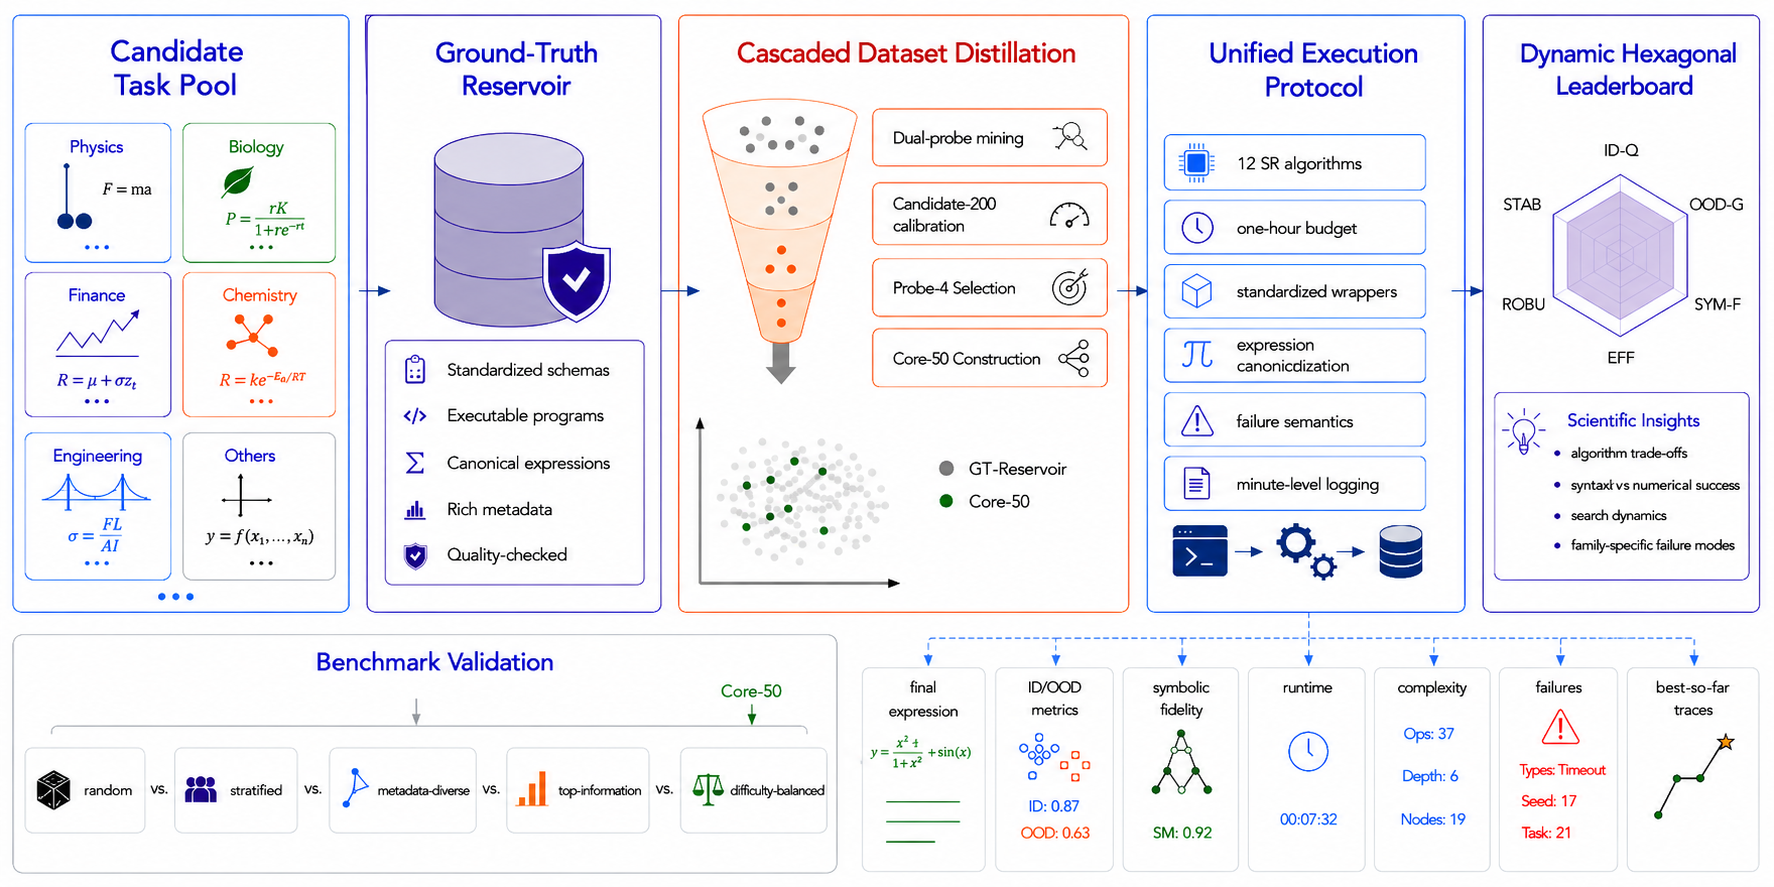
\includegraphics[width=\linewidth]{imgs/Article/figure01_pipeline}
% \caption{\textbf{Overview of \arena{}}. A heterogeneous symbolic regression task pool is standardized into a quality-checked ground-truth reservoir, then a compact and high-information Core-50 benchmark is distilled through cascaded dataset selection. It is evaluated under a unified execution protocol to produce a dynamic six-axis leaderboard and fine-grained search traces. }
% \label{fig:symbolicarena-pipeline}
% \end{figure}


% %
% %\paragraph{Dataset reservoir.}
% %The dataset layer converts heterogeneous SR sources into a shared executable format. Each task has train, validation, ID test, and OOD test splits when available, a ground-truth expression, metadata for structural analysis, and a canonical identity used for semantic duplicate control. This layer is essential because benchmark compression is only meaningful when the larger pool is itself auditable and consistently runnable.
% %
% %\paragraph{Algorithm panel.}
% The algorithm layer integrates 12 representative SR methods across evolutionary, reinforcement-learning, tree-search, neural-guided, transformer, and LLM-assisted families. Every wrapper receives the same data contract, including feature names, target names, dimensionality, budget, seed, and output path. Each run writes a canonical result artifact with status, failure reason, expression, numerical metrics, complexity, runtime, and progress snapshots when available.

% \paragraph{Execution infrastructure.}
% \arena{} uses a layered execution design rather than calling algorithm repositories directly from the benchmark script. A lightweight front-end regressor resolves the requested tool, launches the corresponding wrapper in its configured conda environment, and communicates through JSON commands. The benchmark runner is responsible for loading standardized datasets, injecting the explicit data contract, applying the shared budget and seed, computing train/validation/ID/OOD metrics, exporting canonical symbolic artifacts, and writing result and progress files. This design isolates incompatible dependencies while keeping the result schema and failure semantics identical across methods; implementation details for the execution stack, wrapper contract, result-recovery logic, and data-cleaning pipeline are provided in \cref{app:infra-cleaning}.

% \paragraph{\core{} distillation engine.}
% The distillation layer separates two roles that are often conflated in benchmark construction. The first role is \emph{candidate discovery}: identifying tasks that expose informative method differences. \arena{} performs this with PySR and LLM-SR as two complementary single-seed probes. The second role is \emph{core selection}: choosing a compact benchmark whose structure and response patterns remain representative of the full reservoir. \arena{} performs this with four non-LLM probes selected from the 12-algorithm calibration panel, then runs them on the full 664-task reservoir with three seeds.

% \paragraph{Dynamic leaderboard engine.}
% The leaderboard layer evaluates submitted algorithms on \core{} under a fixed one-hour budget and five seeds. Unlike static final-score tables, \arena{} stores best-so-far expressions at minute resolution. This makes it possible to compare algorithms by final quality, anytime efficiency, symbolic recovery, complexity growth, robustness, and seed stability. Since the six leaderboard axes are normalized against fixed absolute definitions rather than the current set of competitors, adding a new algorithm does not change the previously reported scores.

% \paragraph{Design principle.}
% \arena{} is deliberately not optimized to make all methods win equally. Its goal is to preserve informative differences among methods while keeping the evaluation cost low enough for repeated use. This leads to a benchmark design that balances coverage, discriminability, redundancy control, difficulty, and stability, instead of selecting only the largest-gap or easiest-to-run tasks.
\section{\arena{} Overview}

\arena{} is organized around the evaluation loop summarized in \cref{fig:symbolicarena-pipeline}: a heterogeneous SR task pool is standardized into an auditable ground-truth reservoir, distilled into a compact Core-50 benchmark, evaluated under a unified execution protocol, and reported through a dynamic six-axis leaderboard.

\begin{figure}[t]
\centering
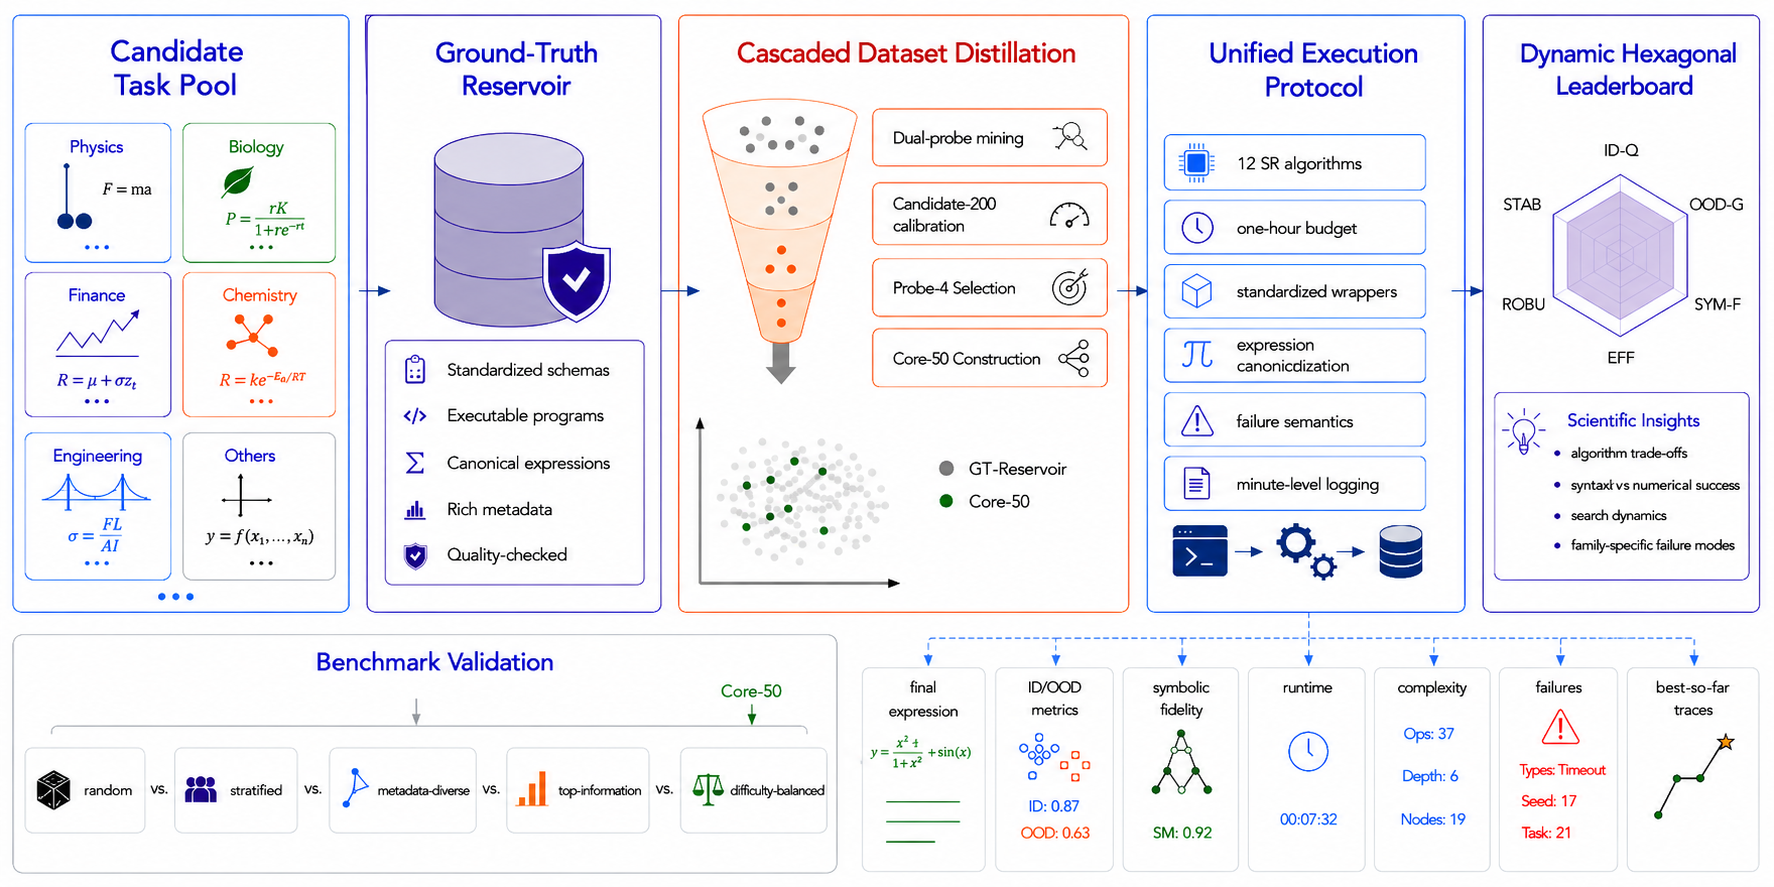
\includegraphics[width=\linewidth]{imgs/Article/figure01_pipeline}
\caption{\textbf{Overview of \arena{}}. A heterogeneous symbolic regression task pool is standardized into a quality-checked ground-truth reservoir, from which a compact and high-information Core-50 benchmark is distilled through cascaded dataset selection. The frozen Core-50 is evaluated under a unified execution protocol to produce a dynamic six-axis leaderboard and fine-grained search traces.}
\label{fig:symbolicarena-pipeline}
\end{figure}

\paragraph{Dataset reservoir.}
The dataset layer converts heterogeneous SR sources into a shared executable format. Each task is associated with standardized data splits, a ground-truth expression, structural metadata, and a canonical identity for semantic duplicate control. This standardized reservoir makes benchmark compression auditable: Core-50 is distilled from a consistently runnable and inspectable task pool rather than from loosely collected datasets.

\paragraph{Algorithm panel and execution protocol.}
The algorithm layer integrates 12 representative SR methods spanning evolutionary search, reinforcement learning, tree search, neural-guided search, transformer-based methods, and LLM-assisted approaches. Each method is accessed through a standardized wrapper that receives the same data contract, budget, seed, and output specification. A lightweight execution layer isolates method-specific environments while enforcing a common result schema, failure semantics, metric computation, expression canonicalization, and progress logging. Implementation details are provided in \cref{app:infra-cleaning}.

\paragraph{\core{} distillation engine.}
The distillation layer separates candidate discovery from final core selection. Candidate discovery uses PySR and LLM-SR as complementary single-seed probes to identify tasks that expose informative differences between classical and LLM-assisted SR methods. Core selection then uses four non-LLM probes, selected from the 12-algorithm calibration panel, to evaluate the full 664-task reservoir with three seeds. The final Core-50 is selected under constraints that balance structural coverage, response diversity, discriminability, redundancy control, difficulty, and stability.

\paragraph{Dynamic leaderboard engine.}
The leaderboard layer evaluates algorithms on the frozen \core{} under a fixed one-hour budget and five random seeds. In addition to final outputs, \arena{} stores best-so-far expressions at minute resolution, enabling analysis of anytime performance, symbolic recovery, complexity growth, robustness, and seed stability. The six leaderboard axes are normalized using fixed absolute definitions rather than relative ranks, so adding new algorithms does not change previously reported scores.

\paragraph{Design principle.}
\arena{} is designed to preserve informative differences among SR methods while keeping evaluation cost low enough for repeated use. The benchmark therefore does not simply select the easiest, hardest, or largest-gap tasks; instead, it distills a compact core that remains representative, discriminative, non-redundant, and stable under repeated evaluation.
